% !TEX encoding = UTF-8
% !TEX TS-program = pdflatex
% !TEX root = ../relazione-finale.tex

%**************************************************************
\chapter{Introduzione}
\label{cap:introduzione}
%**************************************************************

\intro{Nelle sezioni di questo capitolo parlerò dell'idea alla base dello svolgimento dello stage e dei rischi derivati dalle scelte effettuate.}\\

% \noindent Esempio di utilizzo di un termine nel glossario \\
% \gls{api}. \\
% 
% \noindent Esempio di citazione in linea \\
% \cite{site:agile-manifesto}. \\
% 
% \noindent Esempio di citazione nel pie' di pagina \\
% citazione\footcite{womak:lean-thinking} \\

%**************************************************************
\section{L'idea}

Internet Of Things è un paradigma tecnologico diffusosi nell'ultimo decennio. Questa locuzione fa riferimento a un insieme di oggetti,
di varia natura e utilizzo, che interagiscono tra loro e che permettono all'utente di interagire con essi.
L'idea che mi ha spinto allo sviluppo e alla realizzazione del progetto di stage è stata quella unificare in un unico centro di controllo
tutti gli eventuali dispositivi connessi alla rete domestica dell'utente, permettendo 
tuttavia allo stesso di accedere all'interfaccia proprietaria di ciascun dispositivo.
L'obiettivo di una tale dashboard non è quindi \textit{intrappolare} l'utente in un unico ecosistema domotico, 
bensì quello di facilitare la consultazione delle informazioni più frequentemente richieste dall'utente provenienti da più ecosistemi distinti.

Per assicurare prestazioni, affidabilità (\textit{availability}) e scalabilità del prodotto sviluppato e per aggiungere una natura formativa al progetto di stage,
ho scelto di progettare il prodotto secondo l'architettura a microservizi.

\subsection{IoT}

L'idea di una rete di dispositivi smart fu presa in considerazione fin dal 1982, quando un distributore automatico di bibite dell'Università di Carnegie Mellon venne opportunamente modificato per accedere al suo inventario di bibite. Quel distributore automatico divenne il primo apparecchio collegato ad Internet.
\footcite{site:mellon-uni}

Nel corso degli anni '90 il mondo accademico e il mondo dell'industra legata alla produzione continuarono a sperimentare evolvendo il \textit{concept} iniziale, arrivando alla conclusione che l'\textit{Ubiquitous Computing} non si debba riferire solamente ai \textit{computer}, ma debba espandersi agli oggetti di utilizzo quotidiano. Questa visione dovette scontrarsi con i limiti della microelettronica di allora: la produzione di semiconduttori non era ancora pronta a supportare la potenziale domanda e i costi per sostenere l'ampliamento degli impianti non erano facilmente assorbibili in breve tempo. 
\footcite{site:mit-weiser}

Il termine \textit{"Internet of Things"} fu coniato da Kevin Ashton nel 1999.
\footcite{site:iot-kashton}
L'origine dell'espressione, riassumendo le parole dell'autore, deriva dal fatto che la maggior parte delle informazioni presenti su Internet sono state e sono inserite da utenti "umani", soggetti quindi a concentrazione, precisione e tempo limitate;
se queste informazioni fossero invece inserite da macchine senza l'aiuto di un utente umano, la maggior qualità delle stesse garantirebbe
\begin{itemize}
  \item maggiore capacità di tracciamento delle risorse;
  \item minor spreco di risorse;
  \item minor costo per la gestione delle risorse.
\end{itemize}

Grazie agli avanzamenti nei processi di produzione dei semiconduttori, dovuti alla crescita dei mercati del consumo di massa, allo sviluppo di un numero sempre maggiore di tecnologie volte a migliorare l'efficienza e l'affidabilità dei circuiti integrati e alla sempre maggior diffusione di tecnologie per la trasmissione di informazioni senza fili, dai primi anni 2000 il concetto alla base dell'IoT è stato sviluppato da un numero sempre maggiore di aziende negli ambiti più disparati (\textit{home automation}, \textit{manufacturing}, \textit{smart agriculture}, etc.). 
\footcite{site:pc-to-things}

Con Internet of Things si intende una rete di dispositivi interconnessi, individuabili in modo univoco e che possono comunicare informazioni.
I dispositivi presenti in una rete possono comunicare con due tipologie di attori diverse:
\begin{itemize}
  \item se la comunicazione avviene con altri dispositivi si parla di comunicazione M2M (\textit{Machine to Machine}, ovvero comunicazione tra macchine);
  \item se la comunicazione avviene interagendo con il mondo reale si parla di comunicazione M2H (\textit{Machine to Human}, ovvero comunicazione tra macchina e utente).
\end{itemize}

Il termine "Things" nel contesto IoT si riferisce a una varietà di dispositivi come ad esempio: videocamere di sorveglianza, automobili a guida autonoma e assistita oppure piccoli e grandi elettrodomestici casalinghi. Questi dispositivi, soprannominati anche \textit{smart object}, raccolgono informazioni utili in base agli attori con cui comunicano:
\begin{itemize}
  \item se i dispositivi comunicano in modo M2M, le informazioni vengono impiegate al supporto di tecnologie esistenti, integrandosi nel flusso di informazioni esistente; 
  \item se i dispositivi comunicano in modo M2H, le informazioni vengono in aiuto delle persone che interagiscono con essi.
\end{itemize}

L'interesse verso il tema IoT è cresciuto esponenzialmente sia nel mercato consumer che in quello enterprise e secondo Forbes (\footcite{site:forbes-iot}) diventerà nel prossimo quinquennio uno dei settori dell'ITC più redditizi.
É interessante osservare anche la popolarità dei termini di ricerca correlati all'IoT: i dati sono stati ottenuti interrogando il servizio \url{https://trends.google.com/trends}, il quale consente di effettuare analisi sulla popolarità delle stringhe di ricerca immesse nel motore di ricerca di Google.
Ciascun grafico a linea (\textit{line chart} in inglese) presenta nelle ordinate il grado di popolarità della \textit{query} di ricerca, valutato da 0 (popolarità minima) a 100 (popolarità massima), e nelle ascisse l'arco temporale in analisi. 

\begin{figure}[!ht]
    \centering
    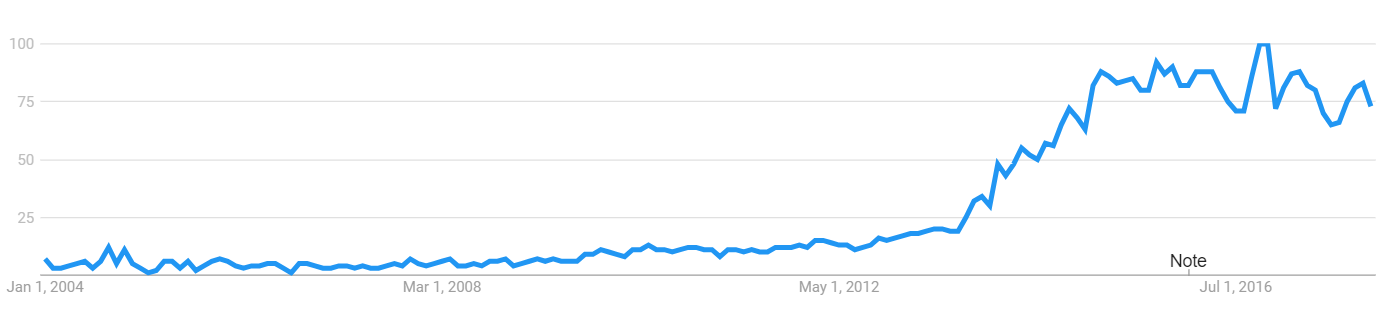
\includegraphics[width=0.9\columnwidth]{intro/internet-of-things-query-interest-worldwide}
    \caption{Andamento dell'interesse per la stringa di ricerca \textit{"internet of things"}. \\ \cite{site:iot-long-trend}}
    \label{fig:internet-of-things-query-interest}
\end{figure}

\begin{figure}[!ht]
    \centering
    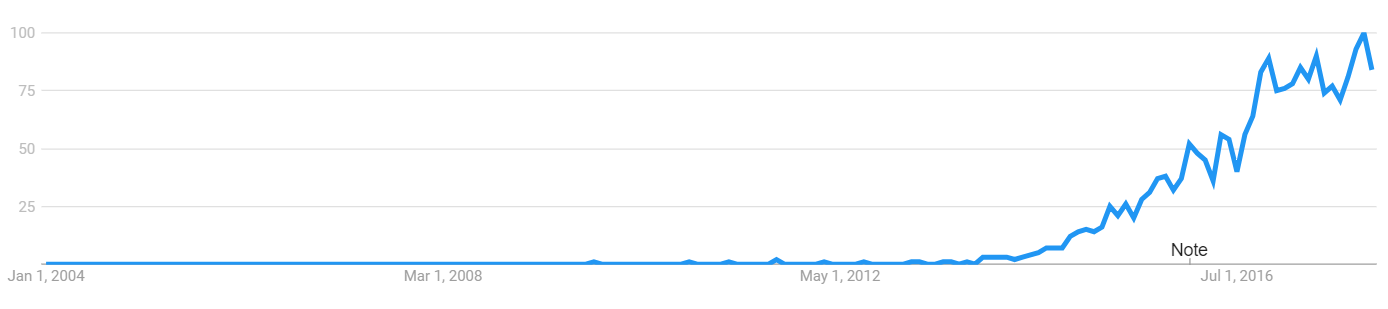
\includegraphics[width=0.9\columnwidth]{intro/iot-devices-query-interest-worldwide}
    \caption{Andamento dell'interesse per la stringa di ricerca \textit{"iot devices"}. \\ \cite{site:iot-devices-trend}}
    \label{fig:iot-devices-query-interest}
\end{figure}

\begin{figure}[!ht]
    \centering
    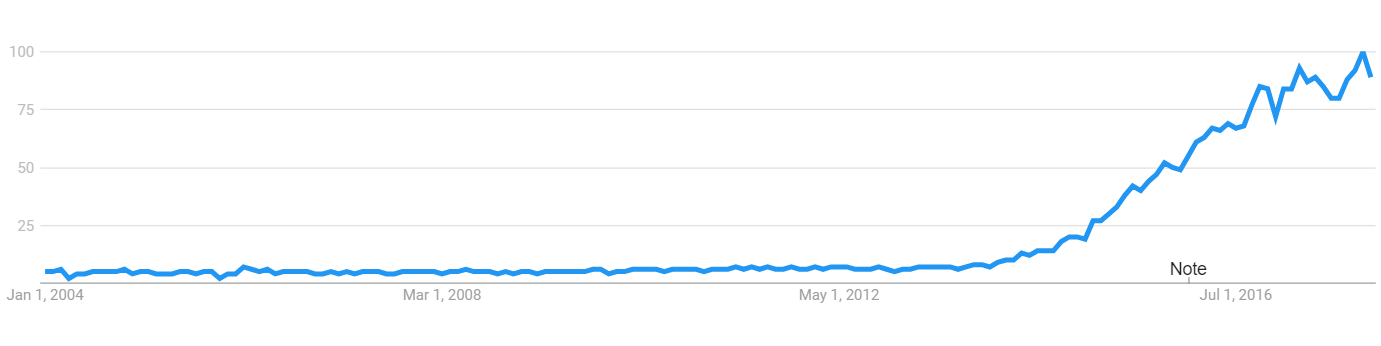
\includegraphics[width=0.9\columnwidth]{intro/iot-query-interest-worldwide}
    \caption{Andamento dell'interesse per la stringa di ricerca \textit{"iot"}. \\ \cite{site:iot-short-trend}}
    \label{fig:iot-query-interest}
\end{figure}

Sintetizzando le previsioni di Forbes con l'andamento dei termini di ricerca legati all'IoT, visibili alle figure ~\ref{fig:internet-of-things-query-interest}, ~\ref{fig:iot-devices-query-interest} e ~\ref{fig:iot-query-interest}, si può notare come l'interesse verso l'argomento IoT stia generalmente aumentando o nel caso peggiore resti stabile con l'interesse degli anni precedenti.

\subsection{Architettura a microservizi}

Illustrare cosa è l'Architettura a microservizi (fornendo un background informativo) e perchè è stato scelto questo tema.

%**************************************************************
\section{Rischi}

Illustrare i rischi derivati dalle scelte effettuate.

%**************************************************************
\section{Organizzazione del testo}

\begin{description}
    \item[{\hyperref[cap:processi-metodologie]{Il secondo capitolo}}] descrive ...

    \item[{\hyperref[cap:descrizione-stage]{Il terzo capitolo}}] approfondisce ...

    \item[{\hyperref[cap:analisi-requisiti]{Il quarto capitolo}}] approfondisce ...

    \item[{\hyperref[cap:progettazione-codifica]{Il quinto capitolo}}] approfondisce ...

    \item[{\hyperref[cap:verifica-validazione]{Il sesto capitolo}}] approfondisce ...

    \item[{\hyperref[cap:conclusioni]{Nel settimo capitolo}}] descrive ...
\end{description}

Riguardo la stesura del testo, relativamente al documento sono state adottate le seguenti convenzioni tipografiche:
\begin{itemize}
	\item gli acronimi, le abbreviazioni e i termini ambigui o di uso non comune menzionati vengono definiti nel glossario, situato alla fine del presente documento;
	\item per la prima occorrenza dei termini riportati nel glossario viene utilizzata la seguente nomenclatura: \emph{parola}\glsfirstoccur;
	\item i termini in lingua straniera o facenti parti del gergo tecnico sono evidenziati con il carattere \emph{corsivo}.
\end{itemize}
